We recommend using categories \bxpref{TasksTCCats} to structure the \gdtestcasebrowser{}. This makes your keywords easier to find when you are creating tests. 

We recommend using two main categories to organize the \gdtestcasebrowser{}: executable tests and modules. 

\subsubsection{Executable tests}
The \bxname{executable test} category contains the following:
\begin{description}
\item [The executable use cases]{as described in \bxpref{BPKeywordSuites}}
\item [A subcategory called \bxname{\gdehandlers{}}]{which is discussed later \bxpref{BPEHandlers}}.
\item [Any tests which reproduce errors]{ from the bug-tracking system, called \bxname{ticket tests}. Each ticket \gdcase{} is named with the ticket number to link it to the bug-tracking system. }
\end{description}

\subsubsection{Modules}
The \bxname{modules} category contains two subcategories: \bxname{AUT-bound modules} and \bxname{unbound modules}. 

\textbf{\gdaut{}-bound modules}\\
This category contains keywords that you have created to perform specific actions in your \gdaut{}. The \gdaut{}-bound modules category is split up into further categories, representing the dialogs and windows of your \gdaut{}. A typical structure for the \gdaut{}-bound modules category might look like this:
\begin{itemize}
\item Dialogs
\begin{itemize}
\item Error Dialogs
\item Load Project Dialog
\item New Project Dialog
\begin{itemize}
\item Configure Language Page
\item Configure Project Page
\end{itemize}
\item Save Dialog
\end{itemize}
\item Main Window
\begin{itemize}
\item General Tab
\item Security Tab
\end{itemize}
\end{itemize}

In each category, the \gdcases{} that execute actions in this area are stored. In the \bxname{Main Window} category, keywords to open dialogs from the menu or the toolbar could be stored. In the \bxname{Main Window - General Tab} category, you would find the keyword to select the security tab, to save the changes in the security tab etc. 

The  \gdaut{}-bound modules are all linked to the \gdaut{} in some meaningful way. For example, they could contain one or more of the following:
\begin{itemize}
\item sequences of actions specific to this \gdaut{}
\item data and/or references specific to this \gdaut{}
\item component names specific to this \gdaut{}
\end{itemize}

Structuring the \gdaut{}-bound modules in this way (\bxfigref{ModulesCategory}) makes it easy to navigate through the keywords you have created. \\


\textbf{Unbound modules}\\
The \bxname{unbound modules} category contains modules which do not fit into the \gdaut{}-bound modules category. Good candidates for the unbound modules are utility modules, as mentioned in the previous section \bxpref{BPKeywordsUtility}. 
Other unbound modules could be sequences of actions that other \gdauts{} could also use. Unbound modules generally contain no data or component names specific to one \gdaut{}. They may, however, contain default data you expect to use throughout your tests (like the operator, the pre-ascend in trees etc). At some point, the unbound modules could be moved into an external \gdproject{} to serve as a library \gdproject{} for more than one \gdaut{} \bxpref{movetoexternal}. 

The unbound module category (\bxfigref{ModulesCategory}) can be structured in categories according to actions or components.


\bxtipp{Think about how many ''layers'' you need in your hierarchy -- sometimes it is well worth making an unbound module, sometimes an unbound module would add an unnecessary extra layer. If your unbound module is not significantly different from the \bxname{ub\_\gdcase{}} from the library \gdproject{}, it is probably superfluous.}

\begin{figure}[h]
\begin{center}
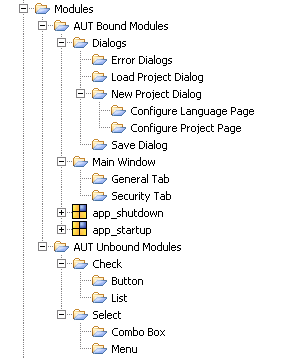
\includegraphics{BestPractices/Structure/PS/ModulesCategory}
\caption{The Modules Category}
\label{ModulesCategory}
\end{center}
\end{figure} 
